%\chapter{Fundamentos de Futebol de Robôs, Sistemas Multi-Agente e Planejamento de Trajetória}
\chapter{Fundamentos de robótica e planejamento de trajetória}
\label{chap:fundam}
O objetivo deste capítulo é fazer uma contextualização do modelo desenvolvido descrevendo as principais abordagens 
de Sistemas Multi-Agente (SMA), seus principais benefícios, tanto dentro como fora da área da robótica. Neste capítulo também 
é feito uma elucidação do conceito de planejamento de trajetória e alguns trabalhos relacionados. Além disso, 
é feita uma descrição de plataformas utilizadas no desenvolvimento de pesquisa na área de robótica no contexto de futebol 
de robôs em ambiente simulado.

Na Seção \ref{sec:sma} é feita uma descrição do conceito de SMA e os principais benefícios de sua 
utilização. São também introduzidos conceitos de comunicação em SMA na sub Seção \ref{subsec:comsma}. 
Por fim, na sub Seção \ref{subsec:coosma} são descritos os tipos de coordenação em SMA e o tipo de 
coordenação utilizada no BahiaRT para alcançar o objetivo deste projeto.

A Seção \ref{sec:futebolderobos} tem como objetivo realizar uma contextualização do objetivo deste trabalho. Na sub Seção
\ref{subsec:ligasdarobocup} é feita uma breve descriçao da RoboCup e algumas ligas padrões definidas como desafios. Na 
sub Seção \ref{subsec:xadrezvsrobocup} é realizada uma abordagem do Xadrez computacional e do futebol de robôs. Nas sub Seçôes 
\ref{subsec:roboviz}, \ref{subsec:simspark} são descritas as plataformas utilizadas na simulação 3D que é descrita na sub Seção 
\ref{subsec:simulacao3d} e posteriormente descrito os principais times campeões dos últimos anos na RoboCup na liga de simulação 3D 
na sub Seção \ref{subsec:times3d}.

Por último, a Seção \ref{sec:planejamentodetrajetorias} descreve o conceito de planejamento de trajetória, alguns trabalhos 
relacionados e os desafios em aberto.

\section{Sistemas Multi-Agente (SMA)}
\label{sec:sma}
Um SMA é um sistema composto por múltiplos agentes interagindo em um ambiente compartilhado. Cada agente
tem a capacidade de agir de forma autônoma tomando decisões que o levarão a atingir o seu objetivo. A interação entre os agentes 
pode ser realizada através de protocolos que são baseados em comportamentos humano. Tal interação tem como objetivo realizar a 
coordenação, cooperação, competição ou negociação dos agentes \cite{reisTese}.

Os SMA tem como objetivo resolver um problema de forma distribuída, aumentando a eficiência da resolução de um problema. Existem 
diversos fatores que demonstram que a utilização de SMA podem trazer benefícios para resolver determinados problemas \cite{stone}:

\begin{enumerate}
 \item O paralelismo, atribuindo diferentes tarefas a diferentes agentes de forma que sua execução seja mais rápida;
 \item A robustez, pois utilizam-se diferentes agentes, não existindo desta forma um ponto único de falha no sistema;
 \item A escalabilidade, permitindo o aumento de agentes de um determinado sistema aberto;
 \item A simplificação das tarefas individuais, dividindo o problema global em subproblemas;
 \item A manutenção da privacidade da informação e conhecimentos individuais de cada agente.
\end{enumerate}

Na Inteligência Artificial (IA), a utilização de SMA trazem diversos benefícios, principalmente da rentabilidade de recursos para 
problemas onde o conhecimento ou atividade é distribuída:

\begin{enumerate}
 \item Resolução mais rápida de problemas por conta do processamento concorrente;
 \item Diminuição da comunicação devido ao processamento estar localizado junto á fonte de informação e a comunicação ser realizada em alto-nível;
 \item Aumento da flexibilidade e escalabilidade resultantes da possibilidade de interconexão de múltiplos sistemas com arquiteturas
 distintas;
 \item Facilidade de desenvolvimento do sistema devido a modularidade resultante da decomposição dos problemas e da decomposição dos 
 sistemas em agentes semi-autônomos.
\end{enumerate}

\subsection{Comunicação em SMA}
\label{subsec:comsma}
Um agente possui a capacidade de percepção, processamento e atuação em um determinado ambiente. Desta forma, a capacidade de se 
comunicar é considerada como um módulo de comunicação, que é dividido em percepção (recepção das mensagens) e de ação (envio de mensagens).
Este módulo está ligado diretamente ao módulo central do agente (módulo inteligente), que permite o agente ter acesso as mensagens 
recebidas do servidor e definir quais as mensagens devem ser enviadas. Uma arquitetura de um agente deliberativo (ou híbrido) com capacidade 
de comunicação pode ser visto na figura \ref{fig:arqComm}.

\begin{figure}[!htb]
\centering
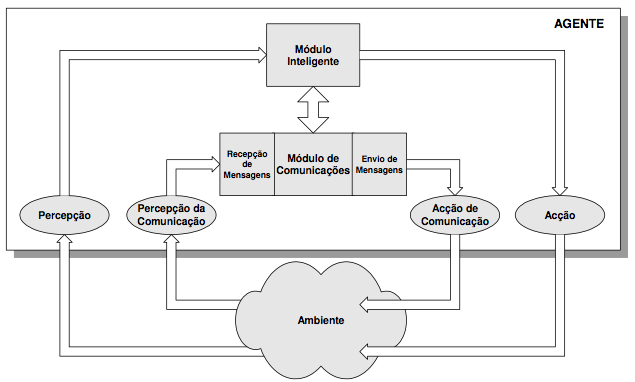
\includegraphics[scale=0.7]{figuras/arquiteturaComm.png}
\caption{Arquitetura de um agente com capacidade de comunicação.} Fonte: \cite{reisTese} \label{fig:arqComm}
\end{figure}
\FloatBarrier

\subsection{Coordenação em SMA}
\label{subsec:coosma}
O Futebol Robótico em geral e a liga de simulação em particular, constituem domínios particularmente adequados a aplicação da 
investigação realizada em metodologias de coordenação em SMA, nomeadamente no que diz respeito a coordenação
para agentes cooperativos \cite{reisTese}.

O domínio do futebol robótico é complexo, dinâmico, parcialmente cooperativo e parcialmente adverso. Existem diversos
tipos de coordenação aplicados ao domínio do futebol robótico. Neste trabalho só será descrito o tipo de coordenação que está sendo 
utilizado no desenvolvimento do modelo, porém a descrição dos diversos tipos de coordenação poderão ser encontradas 
em \citeonline{reisTese}. A coordenação pode ser:

\begin{enumerate}
\item Coordenação por Comunicação.
\item Coordenação por Percepção Inteligente,
\item Coordenação por Modelização Mútua.
\item Coordenação Estratégica.
\item Coordenação Parcialmente Hierarquica.
\end{enumerate}

O tipo de coordenação utilizada neste modelo é focada na coordenação por comunicação. A coordenação por comunicação utiliza um protocolo
que permite que os agentes possam trocar informações acerca do seu estado de mundo e outras informações úteis para a coordenação. Este 
protocolo é baseado no envio de mensagens através de um canal de comunicação entre o agente e o servidor.

A baixa largura de banda do domínio e as restrições impostas à comunicação, são fatores que tornam o futebol robótico simulado um domínio 
atraente para a aplicação de metodologias de coordenação por comunicação.

O time BahiaRT do ACSO, além de utilizar coordenação por comunicação, utiliza a coordenação estratégica. Este tipo de coordenação utiliza 
como premissa a organização dos agentes de tal forma que eles possam definir uma estratégia para um dado jogo, ou situação, composta de 
táticas e definição de papéis (tipos de jogadores) especificando o comportamento individual e coletivo dos agentes.

A construção de agentes capazes de balancear a reatividade com a capacidade de deliberação individual e social são fundamentais 
para que os agentes realizem a cooperação. O estado do mundo de um agente estratégico é definido como uma estrutura multi-nivel
contendo desde informações de baixo nível (incluindo as posições, velocidade e orientações dos objetos presentes no mundo), até 
informação de nível estratégico (incluindo informação temporal estratégica que irá permitir a seleção de táticas a serem utilizadas). 
Este estado de mundo é atualizado utilizando informação proveniente da percepção do agente, das comunicações recebidas (mensagens), da 
dinâmica do mundo e da predição dos efeitos das suas ações e das ações dos outros agentes.

\section{Futebol de Robôs}
\label{sec:futebolderobos}
A iniciativa RoboCup \cite{kitano95} \cite{Kitano97} é um projeto de investigação e educação internacional que tem como objetivo 
promover a investigação em Inteligência Artificial Distribuída (IAD) e Robótica Inteligente \cite{robocup}. O projeto tem como base a 
utilização de um problema padrão – o futebol robótico – onde o desenvolvimento de tecnologias para construir uma equipe de robôs 
reais ou virtuais seja capaz de participar de um desafio de futebol seguindo regras de jogo pré-especificadas.

Como forma de promover a investigação na área, foi lançado um objetivo de longo prazo: 

“No ano de 2050, uma equipe de robôs autônomos humanóides, ser capaz de vencer a 
equipe campeã do mundo de futebol, em uma partida disputada de acordo com as regras da 
FIFA.” \cite{Kitano97} 

Este objetivo é atualmente partilhado como um dos grandes desafios da área da IA e Robótica. 
Embora este desafio, à luz da ciência e tecnologia atuais, pareça altamente ambicioso, a colocação de objetivos científicos
bem definidos de longo prazo, tem sido, ao longo dos anos, uma forma de estimular o desenvolvimento científico \cite{robocup}. 
Além disso, os sub-objetivos que são colocados pela RoboCup através das ligas, convergem para alcançar o objetivo final.

\subsection{Ligas da RoboCup}
\label{subsec:ligasdarobocup}
O futebol robótico inclui diversas ligas que se dividem em dois tipos: ligas robóticas (utilizando robôs pequenos, médios e 
humanóides) e a liga de simulação. O objetivo é fazer com que cada liga se concentre nos desafios propostos, dando ênfase em 
determinados tópicos necessários para fazer com que equipes de robôs possam disputar uma partida de futebol. Por exemplo, 
na liga de simulação, a ênfase é colocada na coordenação em SMA, enquanto na liga de robôs pequenos, a ênfase é colocada no 
controle rápido e preciso dos robôs e na liga de robôs médios, os tópicos mais importantes incluem a visão computacional, 
projeto electromecânico e auto-localização dos robôs.

A RoboCup Rescue \cite{kitano99} e o RoboCup Júnior \cite{sklar02} são também outras iniciativas associadas ao futebol robótico. 
O {\it Rescue} divide-se em robótica física e simulada e tem como objetivo estimular a aplicação da investigação realizada no futebol 
robótico, a domínios socialmente mais úteis, no caso, missões de salvamento e resgate em grandes catástrofes \cite{rescue01}. Já 
a RoboCup Júnior surgiu como uma forma de estimular os mais jovens a participar da RoboCup. A OBR (Olimpíada Brasileira de Robótica) 
é um dos eventos que promovem a inclusão de jovens em idade escolar a construir e colocar em funcionamento os seus robôs para 
realizar diversas tarefas e atraí-los para a CBR (Campeonato Brasileiro de Robótica), que vem atraído a cada ano mais estudantes.

\subsection{Xadrez vs RoboCup}
\label{subsec:xadrezvsrobocup}
Um desafio semelhante colocado aos investigadores em IA no decurso das últimas 4 décadas, consistiu em 
construir um agente (programa) que fosse capaz de vencer o campeão mundial de Xadrez utilizando as regras oficiais da Federação
Internacional de Xadrez. Tal desafio mostrou a importância da existência de problemas padrão em que diferentes metodologias e
avanços científicos podem ser comparados. 

Diversos algoritmos de pesquisa, arquiteturas de computadores e metodologias científicas foram desenvolvidas para este domínio. 
Em Maio de 1997, o computador Deep Blue da IBM \cite{deepblue} derrotou Gary Kasparov (o campeão humano de Xadrez), figura \ref{fig:deepblue}
, utilizando as regras oficiais do Xadrez. Com esta vitória, o desafio de 40 anos da IA utilizando o Xadrez 
como domínio de aplicação ficou muito próximo de um final com sucesso. 

\begin{figure}[!htb]
\centering
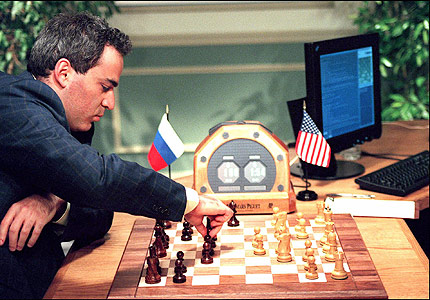
\includegraphics[scale=0.6]{figuras/deepblue.jpg}
\caption{Garry Kasparov x Deep Blue (Computador da IBM), jogando uma partida de Xadrez.} Fonte: \cite{flamencos} \label{fig:deepblue}
\end{figure}
\FloatBarrier

Uma das características que tornou o Xadrez computadorizado um problema padrão foi a facilidade que este domínio ofereceu para
a comparação de abordagens distintas, e para a avaliação do progresso científico global realizado no domínio. No entanto, com a
chegada ao final do desafio associado ao Xadrez, no mundo da IA, novos domínios e problemas padrão mais complexos e estimulantes
tornaram-se necessários. Foi neste contexto que se desenvolveu o desafio do futebol robótico como um problema padrão para a IAD 
e Robótica Inteligente.

As principais diferenças entre o domínio do Xadrez e a RoboCup podem ser visualizadas na tabela \ref{tab:xadrobocup}.

\begin{table}[!htb]

\centering

\caption{Diferenças entre as características dos domínios do RoboCup e Xadrez.} Fonte: \cite{reisTese} 

  \begin{tabular}{|c|c|c|}

    \hline
    \hline
    Caracteristicas / Domínio & Xadrez & RoboCup \\
    \hline
    Ambiente & Estático & Diamico \\
    \hline
    Mudança de Estado & Por turnos & Tempo-Real \\
    \hline
    Acessibilidade ao Estado do Mundo & Completa & Incompleta \\
    \hline
    Resultado das Ações & Determinístico & Não Determinístico \\
    \hline
    Leitura dos Sensores & Discreta (Simbólica) & Contínua (não Simbólica) \\
    \hline
    Utilização dos Atuadores & Discreta (Simbólica) & Contínua (não Simbólica) \\
    \hline
    Controle & Centralizado & Distribuído \\
    \hline
    \hline
  \end{tabular}

  \label{tab:xadrobocup}
\end{table}

A RoboCup foi desta forma projetada de forma a colocar num mundo limitado, um conjunto elevado de complexidades do mundo real, 
mantendo no entanto o custo, complexidade global e dimensão do problema, acessível aos grupos de investigação em Robótica e 
IA. Tais problemas de investigação colocados pela RoboCup de uma forma integrada, cobrem uma vasta área dos 
domínios da IA e Robótica, incluindo: coordenação, cooperação e comunicação multi-agente, arquiteturas de agentes inteligentes, 
aprendizagem, planejamento em tempo-real, decisão estratégica e tática, comportamento reativo, visão computacional, processamento
e análise de imagem, sistemas de locomoção e atuação, sistemas sensoriais, fusão sensorial em tempo-real, navegação, controle 
inteligente robótico e outros.

\subsection{Simulação 3D}
\label{subsec:simulacao3d}
A Simulação 3D de futebol de robôs da RoboCup é uma plataforma que tem como objetivo facilitar o desenvolvimento das pesquisas e 
diminuir o custo com experimentos que os robôs físicos demandam. 

A plataforma se esforça para reproduzir os desafios de 
programação de {\it Software} enfrentdos ao construir robôs físicos reais para esta finalidade. Com a utilização da simulação 3D, 
a investigação encurta o caminho para conseguir atingir a meta da Federação RoboCup de desenvolver uma equipe de robôs humanóides 
totalmente autônomos que possa vencer a equipe campeã mundial de futebol humano em 2050.

\subsection{Simspark}
\label{subsec:simspark}
SimSpark \citeonline{simspark} é um sistema de simulação multi-agente para agentes em ambiente tridimensional desenvolvido como
parte da iniciativa RoboCup. Seu objetivo é fornecer um alto grau de flexibilidade para a criação de novos tipos de simulações. 
Baseia-se em um quadro de aplicação flexível e esgota a idéia de componentes substituíveis ao longo de sua implementação. 

Em comparação com simuladores especializados, os usuários podem criar novas simulações utilizando uma linguagem de descrição de
cena. O SimSpark é uma ferramenta poderosa, pois abrange diferentes questões de investigação multi-agente, e é usado como o 
simulador oficial para a competição {\it RoboCup Simulation League}.

O {\it rcssserver3d} é o ambiente de competição oficial para o {\it Soccer Simulation League} em 3D na RoboCup. Ele implementa uma simulação
de futebol, onde duas equipes de até onze robôs humanóides podem jogar uns contra os outros. Esta configuração aparentemente 
simples, representa um desafio para os implementadores de agentes em vários níveis. 

O modelo de robô utilizado na simulação nas competições é atualmente o NAO, figura \ref{fig:naoColorido}. Contudo, a utilização de agentes
heterogeneos tem ganhado destaque na área científica, que agora querem criar modelos capazes de se adequarem a qualquer tipo de 
robô.

\begin{figure}[!htb]
\centering
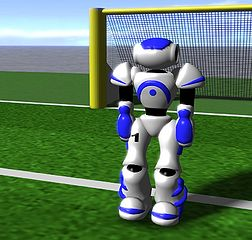
\includegraphics[scale=0.6]{figuras/naoColorido.jpg}
\caption{Simulação do Robô NAO da empresa Aldebaran Robotics feita pelo servidor oficial da liga 3D.} Fonte: \cite{SimulationLeague}. \label{fig:naoColorido}
\end{figure}
\FloatBarrier
              
\subsection{Roboviz}
\label{subsec:roboviz}
RoboViz \citeonline{roboviz} é um programa de {\it Software} projetado para avaliar e desenvolver comportamentos de agentes em sistemas 
multi-agente. RoboViz é um monitor interativo que torna o agente e informações sobre o 
estado do mundo em uma cena tridimensional. Além disso, o RoboViz fornece um design programável e funcionalidade de depuração
para os agentes que podem se comunicar através de uma rede. 

A ferramenta facilita a visualização em tempo real de agentes em execução simultânea no simulador SimSpark, fornecendo uma análise
de nível superior e visualização de comportamentos do agente, figura \ref{fig:roboviz}, que não está atualmente disponível nas 
ferramentas já existentes.

\begin{figure}[!htb]
\centering
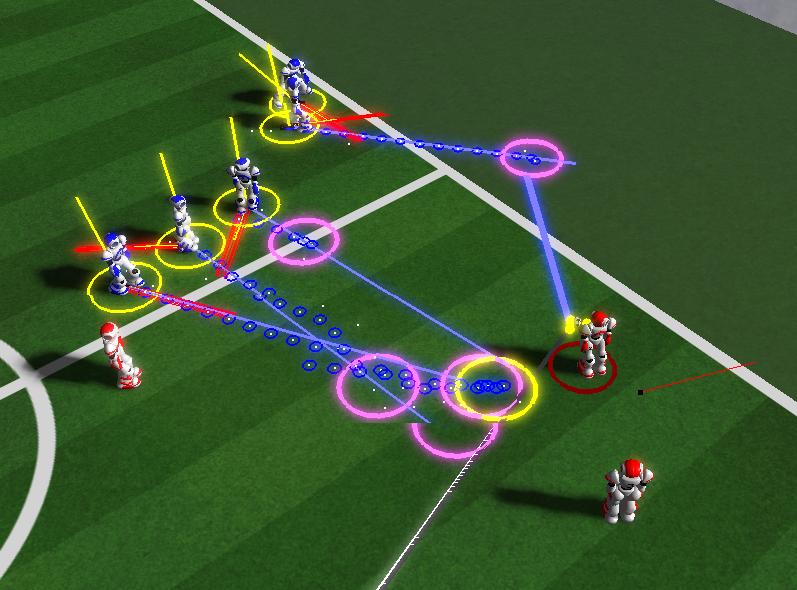
\includegraphics[scale=0.38]{figuras/roboviz.png}
\caption{Simulação em tempo real de agentes no RoboViz utilizando um plot gráfico para analise de comportamentos.} Fonte: \cite{robovizImg} \label{fig:roboviz}
\end{figure}
\FloatBarrier

\subsection{Times da Simulação 3D}
\label{subsec:times3d}
A liga de simulação 3D é composta por times que foram desenvolvidos por grupos de pesquisa de diversos países. A quantidade de
equipes que possuem times competitivos é pequena, isso se da pelo fato de que o desenvolvimento de uma equipe requer uma pesquisa
aprofundada sobre movimentação de agentes, protocolos de comunicação, planejamento e coordenação multi-agente e IAD.

Um dos fatores que facilitam grupos de pesquisa se inserirem na competição, são os códigos de times base disponibilizados por equipes para
fomentar e estimular a pesquisa no \^ambito da robótica autônoma simulada. Como por exemplo, o MagmaOffenburg \cite{magma}, um time
base cedido para a comunidade científica.

Atualmente os principais times que participam da RoboCup podem ser visualizados na tabela \ref{tab:times}.

\begin{table}[!htb]

\scalefont{0.8}
\centering
\caption{Principais times que participam da RoboCup e sua Universidade.} Fonte: \cite{SimulationLeague} 

  \begin{tabular}{|c|c|}
    \hline
    \hline
    Time & Universidade \\
    \hline
    \hline
    Apollo3D & Nanjing University of Posts and Telecommunications \\
    \hline`
    AUA3D & Anhui University of Architecture \\
    \hline
    BahiaRT & Universidade do Estado da Bahia \\
    \hline
    Bold Heart & University of Hertfordshire \\
    \hline
    cit3d & Changzhou Institute of Technology \\
    \hline
    FCPortugal & University of Aveiro/University of Minho/University of Porto \\
    \hline
    FUT-K3D & Fukui University of Technology \\
    \hline
    HfutEngine3D & HFUT \\
    \hline
    ITAndroids & Instituto Tecnologico de Aeronautica \\
    \hline
    IUIM3D & Iran University of Industries Mines (Tehran Center Branch) \\
    \hline
    KarachiKoalas & University of Technology, Sydney and Institute of Business Administration, Karachi \\
    \hline
    KylinSky3D & Hohai University Wentian College / Hohai University \\
    \hline
    L3M-SIM & Paris8 University \\
    \hline
    magmaOffenburg & Hochschule Offenburg \\
    \hline
    Miracle3D & Hefei Normal University \\
    \hline
    Mithras3D & Farzanegan Tehran \\
    \hline
    Nexus3D & Ferdowsi University of Mashhad \\
    \hline
    ODENS & Osaka Electro-Communication University \\
    \hline
    Paydar3D & Sharif University Of Technology \\
    \hline
    Rightel & University of Tehran \\
    \hline
    RoboCanes & University of Miami \\
    \hline
    Scorpius & AmirKabir University of Technology (AUT) \\
    \hline
    SEU-Jolly & Southeast University \\
    \hline
    UTAustinVilla & University of Texas at Austin \\
    \hline
    \hline
  \end{tabular}

  \label{tab:times}
\end{table}


Além dos times base, o TDP ({\it Team Description Paper}), que são descrições de cada time e artigos sobre as metodologias empregadas
em seus times, são divulgadas em simpósios e congressos, facilitando o trabalho de outras equipes e fomentando a melhoria contínua
de metodologias empregadas para resolver problemas em aberto.

Alguns dos problemas em aberto nesta liga são: como fazer com que os agentes corram, fazer 
com que agentes efetuem um passe de forma coordenada e planejada, desviar de obstáculos móveis e atuarem com sucesso em ambi\^entes dinâmicos. 
Um dos times que mais se aproxima da movimentação baseada no comportamento humano é o MagmaOffenburg \cite{dorer}, 
que por sua vez poderá ser um dos primeiros times a conseguir fazer com que o robô consiga correr.

Um outro time que ganhou destaque nas últimas competições foi o UTAustinVilla \cite{MacAlpine2}. Desenvolvido por um grupo de 
estudantes da Universidade de Austin, Estados Unidos, coordenado por Peter Stone, pesquisador renomado na área de robótica. 
Uma das principais características que determinaram o seu sucesso foi a sua movimentação omnidirecional com capacidade de 
se manter estável mesmo colidindo com outros agentes.

O time FCPortugal \citeonline{fcportugal} desenvolvido pelo grupo de pesquisa da Universidade do Porto, Portugal, terceiro lugar na simulação 3D da 
RoboCup 2013, teve como diferencial o seu super chute, capaz de alcançar até 20 metros, mais da metade do campo utilizado pelo servidor 
Simspark. Apesar de ser um chute estático, o seu alcance é fruto da otimização do {\it script} utilizado na perna que realiza o chute.

Na RoboCup de 2013, o time vencedor da simulação 3D foi o Apollo3D \cite{apollo3d}. Uma das principais contribuições que o 
grupo de pesquisa que desenvolveu o Apollo3D vem dispondo a comunidade científica é o seu código fonte.

A maioria dos times hoje utilizam uma movimentação omnidirecional e dinâmica, onde suas poses são calculadas e alcançadas através de 
modelos matemáticos utilizando cinemática inversa. Tais modelos substituiram a movimentação estática, que dificultava a realização de 
jogadas e comportamentos devido o fato de que o ambiente é dinâmico e contínuo. 


\section{Planejamento de trajet\'oria}
\label{sec:planejamentodetrajetorias}
O objetivo principal do planejamento de trajetória é a construção de algoritmos para automatizar o movimento de robôs, 
peças e outros ambientes que utilizam objetos geométricos arbitrários. Uma tarefa básica é mover um robô em seu ambiente de trabalho 
a partir de uma posição e orientação para outra posição e orientação desejada, sem o robô bater em obstáculos. O planejamento de trajetória
tem aplicações tanto dentro, como fora da área de robótica.

O problema de navegação mais básico é mover um robô modelado como um ponto no espaço através de um ambiente bidimensional com vários
itens proibidos (ou obstáculo). O obstáculo é considerado uma região em que o robô não pode entrar. O modelo é cinemático, o que significa
que a única limitação é que o robô tem de se mover ao longo de uma trajetória contínua.

O robô é modelado como um ponto no espaço de configuração, em vez de espaço de trabalho. Uma configuração é uma especificação
do local (localização e orientação) do robô em relação ao meio ambiente e o espaço de configuração é o conjunto de todas as configurações
possíveis \cite{achoset}.

Realizar o planejamento apresenta um maior nível de complexidade quando o robô tem muitos graus de liberdade e orientação. Um robô 
guia pode passar por um espaço com uma certa posição e orientação, e atinge um obstáculo se fosse em uma orientação diferente. Isso 
aumenta a complexidade dos algoritmos para planejamento de trajetória. Além disso, podem existir obstáculos móveis no ambiente, 
aumentando ainda mais a complexidade da busca de uma trajetória eficiênte, sem que haja colisão.

O exemplo clássico de planejamento de trajetória é o problema do mecanismo de enfileiramento \cite{bsharir}: 
mover um piano através de uma casa sem colidir com outros objetos na casa (ou a própria casa). Considerando somente a 
geometria dos objetos e não as forças que atuam sobre o piano, como a gravidade .

Estendendo a analogia, o piano é suposto ter motores infinitamente fortes e infinitamente pequenos. Portanto, o problema do motor 
de piano só lida a circulação de uma forma geométrica ao longo de um caminho que é contínuo no espaço através de uma atmosfera.

Existem diversos algoritmos que tratam da navegação de agentes autônomos, sendo que um dos primeiros é descrito no livro de
Inteligência Artificial de Russell e Norvig, o algorítmo A* \cite{brussel}. Ele busca o caminho em um grafo de
um vértice inicial até um vértice final, é a combinação de aproximações heurísticas como do algoritmo {\it Best-first Search} e da
formalidade do Algoritmo de Dijkstra (DIJKSTRA, 1959). 

A partir do algoritmo A*, surgiram derivações como o R* \cite{plikhachev}, que depende muito menos da qualidade da função heurística, 
evitando mínimos locais e resolvendo o problema de planejamento de toda uma série de pesquisas de curto alcance.